\newpage
\section*{Zielsetzung}
Es soll die Compton-Wellenlänge $\lambda_c$ des Elektrons bestimmt werden
\section{Theorie}
\subsection{Die Compton-Strahlung}
\label{sec:theorie}
Streut Röntgenlicht mit einer Wellenlänge $\lambda_1$ an einem schwach gebunden Elektron, so enthält das gestreute Licht eine neue 
größere Wellenlänge $\lambda_2$, da das Photon einen Teil seiner Energie durch den inelastischen Stoß
an das Elektron übertragten hat. Zusätzlich wird diese Wlennenlänge um den Winkel $\Theta$ abgelenkt.
Die Wellenlängenverschiebung $\Delta \lambda$ und der Streuungswinkel 
$\Theta$ weisen folgenden Zusammhang auf
\begin{equation}
    \Delta \lambda = \lambda_2 - \lambda_1 =\frac{h}{m_e c}\left(1-cos(\Theta)\right)=\lambda_c \cdot \left(1-cos(\Theta)\right).
\end{equation}
Die Konstante nennt man die Compton-Wellenlänge des Elektrons.
\begin{figure}
    \centering
    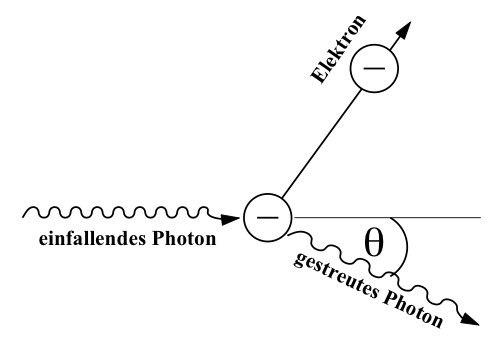
\includegraphics[width=0.4\textwidth]{compton/compton_effekt.jpg}
    \caption{Darstellung des Compton Effekts mit einfallendem Photon, dass
    auf ein Elektron trifft. Das gestreute Photon wird um den Winkel $\Theta$
    abgelenkt.}
\end{figure}

\subsection{Erzeugung der Röntenstrahlung}
Zur Erzeugung nutze man die Eigenschaft der Bremstrahlung sowie die charakteristische
Röntgenstrahlung des Anodenmaterials.\\ 
Eine Glühkathode emittiert dabei Elektronen, die durch eine evakuierte Röhre auf 
eine Annode hin beschleunigt werden. 
Beim Durchlaufen einer Gegenspannung wird das Elektron abgebremst und es wird Energie
in Form eines kontinuierlichen Sprektrums von Röntgenquanten (Photonen) frei. 
Trifft das Elektron schließlich auf das Anodenmaterial auf, so entsteht charakteristische Röntgenstrahlen aufgrund der Ionisierung
des Materials. Die dort gebunden Elektronen können dadurch in innere Schalen zurückfallen und senden Röntgenquanten mit spezifischer
Energie die Materialabhängig ist aus.

Über die Bragg'sch Reflektion kann die Energie $E$ der Strahlung analysiert werden.
Durch die Beugung der Strahlung an einem dreidimensionalen Gitter mit dem Gitterkonstante $d$ 
entsteht beim Glanzwinkel $\alpha$ eine konstruktive Interferenz. Die Wellenlänge bestimmt 
sich nun über den Zusammenhang
\begin{equation}
    2 d sin(\alpha)=n \lambda,
\end{equation}
wobei $n$ die Beugungsordnung beschreibt.


\subsection{Bestimmung Compton-Strahlungscharakteristika}
Um die Compton-Wellenlänge zu bestimmen nutzt man die Transmission und Absorbion durch Aluminium, welche abhängig ist von 
der Wellenlänge.\\
Bei der Absorbion durch ein Materie der Dicke $d$ wird die Intensität $I_0$ nach dem Delamber'schen Gesetz geschwächt
\begin{equation}
    I=I_0e^{-\mu d}.
\end{equation}
wobei $\mu$ den Absorbionskoeffizient beschreibt der sich folgend zusammensetzt
\begin{equation}
    \mu =\mu_{Paar}+\mu_{Photo}+\mu_{Com}.
\end{equation}
\newline

Mithilfe der Transmission, also